% BE-06: Database Schema and API Specification — compile with XeLaTeX (Overleaf: Menu → Compiler → XeLaTeX)
% Put erd.png (export from dbdiagram.io) next to this file to include the ER diagram.
\documentclass[11pt,a4paper]{article}

% ---------- language and fonts ----------
\usepackage{fontspec}
\usepackage{polyglossia}
\setdefaultlanguage{english}
\IfFontExistsTF{Times New Roman}{\setmainfont{Times New Roman}}{%
  \IfFontExistsTF{Liberation Serif}{\setmainfont{Liberation Serif}}{\setmainfont{DejaVu Serif}}}
\IfFontExistsTF{Arial}{\setsansfont{Arial}}{%
  \IfFontExistsTF{Liberation Sans}{\setsansfont{Liberation Sans}}{\setsansfont{DejaVu Sans}}}
\IfFontExistsTF{Consolas}{\setmonofont[Scale=0.88]{Consolas}}{\setmonofont[Scale=0.82]{DejaVu Sans Mono}}

% ---------- layout ----------
\usepackage[margin=2.2cm]{geometry}
\usepackage{microtype}
\usepackage{graphicx}
\usepackage{array}
\usepackage{booktabs}
\usepackage{xltabular}
\usepackage{enumitem}
\usepackage[table]{xcolor}
\usepackage{caption}
\usepackage{float}
\usepackage{fancyvrb}
\usepackage{xurl}
\usepackage[colorlinks=true,linkcolor=blue!50!black,urlcolor=blue!50!black]{hyperref}

\setlist{itemsep=2pt,topsep=4pt}
\setlength{\parskip}{4pt}
\setlength{\parindent}{0pt}
\setlength{\emergencystretch}{3em}
\renewcommand{\arraystretch}{1.25}
\newcolumntype{L}{>{\raggedright\arraybackslash}X}
\newcolumntype{P}[1]{>{\raggedright\arraybackslash}p{#1}}
\newcommand{\tblstart}{\small\rowcolors{2}{gray!7}{white}}
\newcommand{\code}[1]{\texttt{#1}}
\newcommand{\GET}{\textcolor{green!45!black}{\texttt{GET}}}
\newcommand{\POST}{\textcolor{blue!60!black}{\texttt{POST}}}
\newcommand{\PATCH}{\textcolor{orange!80!black}{\texttt{PATCH}}}
\newcommand{\DEL}{\textcolor{red!65!black}{\texttt{DELETE}}}
\fvset{fontsize=\small,frame=single,framesep=5pt,rulecolor=\color{gray!50}}

\title{\textbf{BE-06: Database Schema and API Specification}\\[4pt]
\large Intelligent Kanban System with an AI Assistant}
\author{Symbat Saparbay | Akbope Bakytkeldy\\ \small YouTrack: DEMO-32}
\date{}

\begin{document}
\maketitle
\tableofcontents
\newpage

% =====================================================
\section{Purpose and Scope}

This document defines the data model and the backend API that the MVP will implement. It covers:
\begin{itemize}
  \item the PostgreSQL schema (ER diagram, tables, constraints, indexes);
  \item REST endpoints for authentication, workspaces, projects, boards, tasks, comments and notifications;
  \item the AI command API and the specification of all eight AI actions: input parameters, response structure, validation rules and error handling;
  \item WebSocket events for real-time updates;
  \item a mapping from user stories to endpoints.
\end{itemize}
It builds on BE-03 (technology selection), BE-05 (backend components and AI command life cycle) and the product requirements (PRD).

% =====================================================
\section{Database Schema}

\subsection{ER Diagram}

The editable source of the diagram is \code{docs/be-06/kanban-schema.dbml} (dbdiagram.io); the export below is generated from it.

\IfFileExists{erd.png}{%
\begin{figure}[H]
\centering
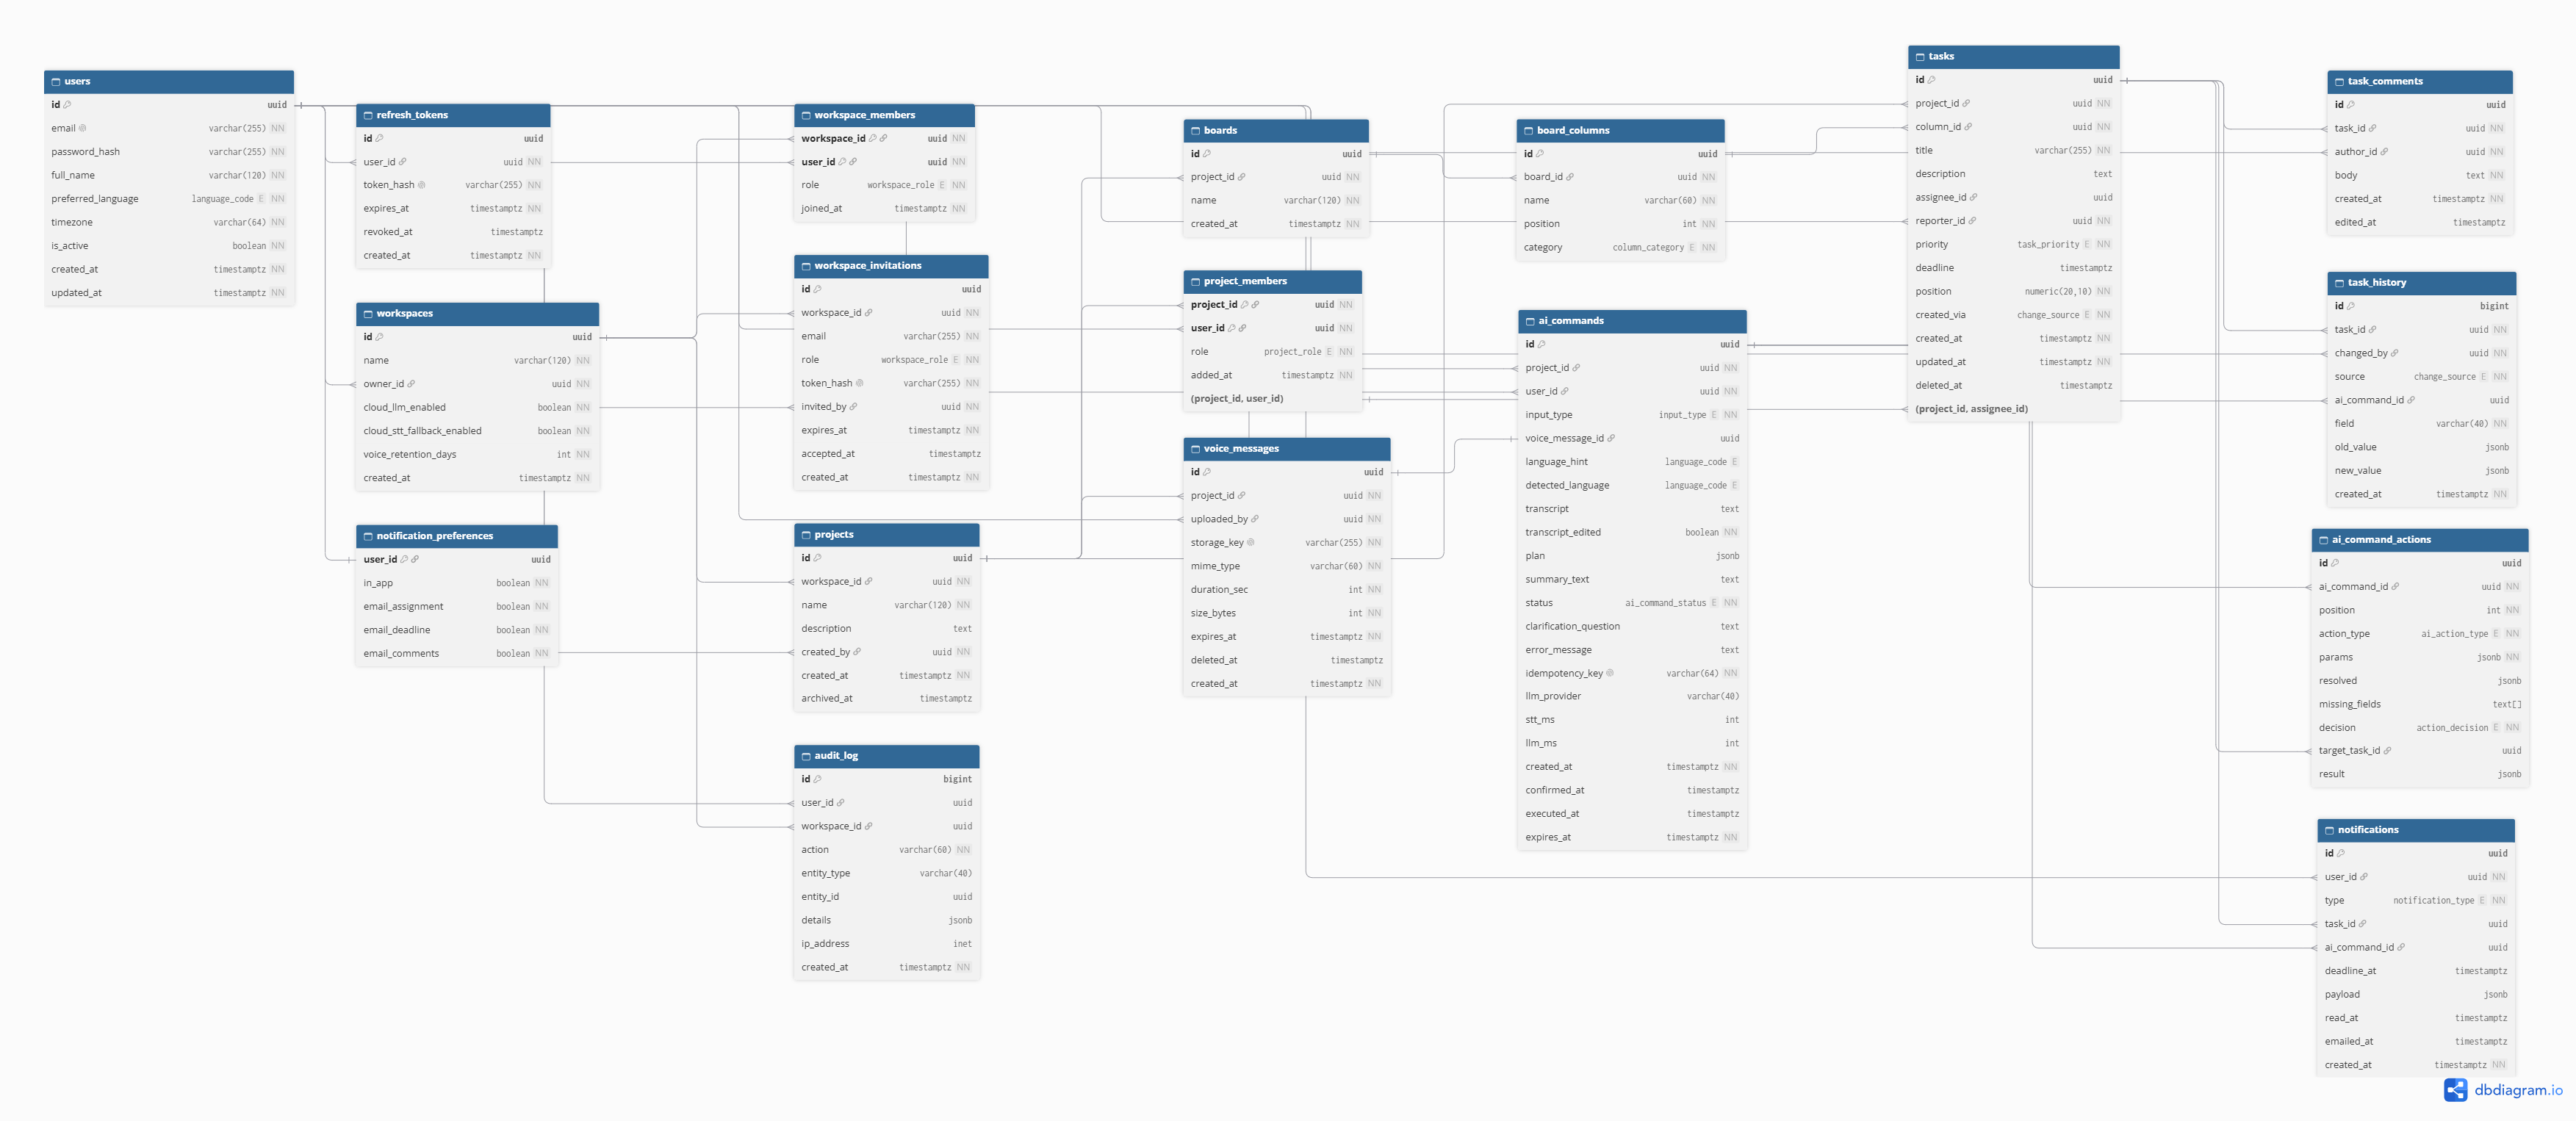
\includegraphics[width=\textwidth,height=0.75\textheight,keepaspectratio]{erd.png}
\caption{Entity--relationship diagram (PostgreSQL 16).}
\end{figure}}{%
\begin{center}\fbox{\parbox{0.9\textwidth}{\centering\small ER diagram: export \code{erd.png} from \code{kanban-schema.dbml} in dbdiagram.io and place it next to this file.}}\end{center}}

\subsection{Tables}

{\tblstart
\begin{xltabular}{\textwidth}{P{4.3cm} L}
\toprule
\textbf{Table} & \textbf{Purpose and key fields} \\
\midrule
\endhead
\multicolumn{2}{l}{\cellcolor{white}\textbf{Users and access}} \\
\code{users} & Account: email (unique), Argon2 password hash, full name, preferred language (kk/ru/en), time zone (used to resolve relative deadlines) \\
\code{refresh\_tokens} & Refresh tokens (hashed), expiry, revocation \\
\code{workspaces} & Workspace with AI settings: \code{cloud\_llm\_enabled} (false = private mode), \code{cloud\_stt\_fallback\_enabled}, \code{voice\_retention\_days} (default 30) \\
\code{workspace\_members} & User--workspace link with role \code{owner}, \code{admin} or \code{member}; primary key (workspace, user) \\
\code{workspace\_invitations} & Email invitations with role, hashed token and expiry \\
\midrule
\multicolumn{2}{l}{\cellcolor{white}\textbf{Projects and boards}} \\
\code{projects} & Project inside a workspace; can be archived \\
\code{project\_members} & User--project link with role \code{manager}, \code{member} or \code{viewer}. AI assignee mentions are resolved only against this table \\
\code{boards} & Boards of a project \\
\code{board\_columns} & Ordered columns with a category \code{todo}, \code{in\_progress} or \code{done}; the category maps any column name to a status \\
\midrule
\multicolumn{2}{l}{\cellcolor{white}\textbf{Tasks}} \\
\code{tasks} & Title, description, assignee (nullable), reporter, priority, deadline, position in column, \code{created\_via} (ui/ai), soft delete. Status is defined by the column. The board is known through the column \\
\code{task\_comments} & Comments with author and time \\
\code{task\_history} & Append-only change log: field, old and new value, author, source (ui/ai), link to the AI command \\
\midrule
\multicolumn{2}{l}{\cellcolor{white}\textbf{Voice and AI}} \\
\code{voice\_messages} & Metadata of an encrypted audio file in MinIO: storage key, MIME type, duration, size, \code{expires\_at} \\
\code{ai\_commands} & One voice or text command: transcript, language hint and detected language, status, plan (JSONB), \code{summary\_text}, clarification question, \code{idempotency\_key} (unique), provider, STT and LLM timings, \code{expires\_at} \\
\code{ai\_command\_actions} & Actions inside a command (one command can contain several): type, spoken parameters, resolved IDs, missing fields, decision (pending/accepted/rejected), target task, result \\
\midrule
\multicolumn{2}{l}{\cellcolor{white}\textbf{Notifications and audit}} \\
\code{notifications} & In-app notifications with type, task, deadline the reminder refers to, read and emailed timestamps \\
\code{notification\_preferences} & Per-user switches for in-app and email notifications \\
\code{audit\_log} & Append-only log of security-relevant actions \\
\bottomrule
\end{xltabular}}

\subsection{Integrity Rules in the Database}

{\tblstart
\begin{xltabular}{\textwidth}{P{4.6cm} L}
\toprule
\textbf{Rule} & \textbf{Implementation} \\
\midrule
\endhead
Assignee must be a project member & Composite foreign key \code{tasks(project\_id, assignee\_id)} $\rightarrow$ \code{project\_members(project\_id, user\_id)}; NULL is allowed \\
Repeated confirmation creates nothing & Unique \code{ai\_commands.idempotency\_key}; confirmation runs in one transaction with a row lock \\
No duplicate deadline reminders & Unique \code{(user\_id, task\_id, type, deadline\_at)} in \code{notifications} \\
Column order & Unique \code{(board\_id, position)} in \code{board\_columns} \\
Delete behaviour & Cascade: workspace $\rightarrow$ projects $\rightarrow$ boards $\rightarrow$ columns; project $\rightarrow$ tasks $\rightarrow$ comments and history. Restrict: a column with tasks, a project member with assigned tasks. Tasks are soft-deleted \\
Fuzzy task search & GIN index with \code{gin\_trgm\_ops} on \code{tasks.title} (extension \code{pg\_trgm}) \\
Overdue and due-soon queries & Index \code{(assignee\_id, deadline)} \\
\bottomrule
\end{xltabular}}

% =====================================================
\section{API Conventions}

{\tblstart
\begin{xltabular}{\textwidth}{P{3.4cm} L}
\toprule
\textbf{Aspect} & \textbf{Convention} \\
\midrule
\endhead
Base URL & \code{/api/v1}; JSON request and response bodies; UTF-8 \\
Authentication & \code{Authorization: Bearer <access\_token>} (JWT, 15 min); refresh token in an httpOnly cookie (30 days) \\
Identifiers & UUID v4 in paths and bodies \\
Dates & ISO 8601 with time zone, e.g. \code{2026-10-23T18:00:00+05:00} \\
Pagination & \code{?limit=50\&cursor=<opaque>}; responses contain \code{items} and \code{next\_cursor} \\
Idempotency & \code{Idempotency-Key} header on \code{POST} requests that create data; AI confirmation is idempotent by design \\
Permissions & Every endpoint checks workspace and project roles (Section~\ref{sec:roles}); inaccessible resources return 404 to avoid revealing their existence \\
Specification & The OpenAPI document is generated by FastAPI at \code{/api/v1/openapi.json}; this document is the agreed design \\
\bottomrule
\end{xltabular}}

\subsection{Error Format}

\begin{Verbatim}
{
  "error": {
    "code": "assignee_not_found",
    "message": "No project member matches \"Данияр\".",
    "details": { "field": "assignee", "candidates": [] }
  }
}
\end{Verbatim}

{\tblstart
\begin{xltabular}{\textwidth}{P{1.5cm} P{4.6cm} L}
\toprule
\textbf{HTTP} & \textbf{Code examples} & \textbf{When} \\
\midrule
\endhead
400 & \code{validation\_error} & Body does not match the schema (wrong type, empty title, unknown priority) \\
401 & \code{unauthorized}, \code{token\_expired} & Missing or invalid token \\
403 & \code{forbidden} & Authenticated but the role does not allow the action (e.g. viewer edits a task) \\
404 & \code{not\_found} & Resource does not exist or is not accessible \\
409 & \code{conflict}, \code{command\_not\_confirmable}, \code{command\_expired} & State does not allow the action (command already rejected, expired, or plan out of date) \\
413 & \code{audio\_too\_large} & Audio larger than 10 MB or longer than 5 minutes \\
415 & \code{unsupported\_audio\_format} & Not one of WebM/Opus, OGG, MP3, WAV, M4A \\
422 & \code{needs\_clarification} & The command cannot be confirmed until missing or ambiguous fields are resolved \\
429 & \code{rate\_limited} & Too many AI commands (limit: 30 per user per minute) \\
503 & \code{ai\_unavailable} & STT and LLM providers (including fallback) are unavailable; manual actions still work \\
\bottomrule
\end{xltabular}}

% =====================================================
\section{Roles and Permissions}\label{sec:roles}

{\tblstart
\begin{xltabular}{\textwidth}{L P{1.6cm} P{1.6cm} P{1.6cm} P{1.6cm}}
\toprule
\textbf{Action} & \textbf{Owner / admin} & \textbf{Manager} & \textbf{Member} & \textbf{Viewer} \\
\midrule
\endhead
Manage workspace settings and members & Yes & No & No & No \\
Create projects, boards, columns; add project members & Yes & Yes & No & No \\
Create and edit tasks, move cards, comment & Yes & Yes & Yes & No \\
Delete tasks & Yes & Yes & Own tasks & No \\
AI actions that change data (create, update, status, assign, deadline, priority) & Yes & Yes & Yes & No \\
AI Search Tasks and Project Summary & Yes & Yes & Yes & Yes \\
View boards and tasks & Yes & Yes & Yes & Yes \\
\bottomrule
\end{xltabular}}

Workspace owners and admins have manager rights in every project of the workspace. AI actions are executed with the permissions of the user who confirms them.

% =====================================================
\section{REST Endpoints}

\subsection{Authentication}
{\tblstart
\begin{xltabular}{\textwidth}{P{1.3cm} P{6.6cm} L}
\toprule
\textbf{Method} & \textbf{Path} & \textbf{Description} \\
\midrule
\endhead
\POST & \code{/auth/register} & Create an account (email, password, full name, language, time zone) \\
\POST & \code{/auth/login} & Returns an access token and sets the refresh cookie; invalid credentials return 401 \\
\POST & \code{/auth/refresh} & New access token from the refresh cookie; rotates the refresh token \\
\POST & \code{/auth/logout} & Revokes the refresh token \\
\GET & \code{/users/me} & Current user profile \\
\PATCH & \code{/users/me} & Update name, language, time zone, notification preferences \\
\bottomrule
\end{xltabular}}

\subsection{Workspaces and Members}
{\tblstart
\begin{xltabular}{\textwidth}{P{1.3cm} P{6.6cm} L}
\toprule
\textbf{Method} & \textbf{Path} & \textbf{Description} \\
\midrule
\endhead
\GET & \code{/workspaces} & Workspaces of the current user \\
\POST & \code{/workspaces} & Create a workspace; the creator becomes owner \\
\PATCH & \code{/workspaces/\{id\}} & Rename; AI settings (cloud LLM, STT fallback, voice retention) \\
\GET & \code{/workspaces/\{id\}/members} & Members with roles \\
\POST & \code{/workspaces/\{id\}/invitations} & Invite by email with a role \\
\POST & \code{/invitations/\{token\}/accept} & Accept an invitation \\
\PATCH & \code{/workspaces/\{id\}/members/\{user\_id\}} & Change role (owner/admin only) \\
\DEL & \code{/workspaces/\{id\}/members/\{user\_id\}} & Remove a member (fails with 409 if they still have assigned tasks) \\
\bottomrule
\end{xltabular}}

\subsection{Projects, Boards and Columns}
{\tblstart
\begin{xltabular}{\textwidth}{P{1.3cm} P{6.6cm} L}
\toprule
\textbf{Method} & \textbf{Path} & \textbf{Description} \\
\midrule
\endhead
\GET & \code{/workspaces/\{id\}/projects} & Projects accessible to the user \\
\POST & \code{/workspaces/\{id\}/projects} & Create a project with a default board (To Do, In Progress, Done) \\
\GET / \PATCH & \code{/projects/\{id\}} & Read or update (name, description, archive) \\
\GET & \code{/projects/\{id\}/members} & Project members with roles \\
\POST & \code{/projects/\{id\}/members} & Add a workspace member to the project with a role \\
\PATCH / \DEL & \code{/projects/\{id\}/members/\{user\_id\}} & Change role or remove \\
\GET & \code{/projects/\{id\}/boards} & Boards of the project \\
\GET & \code{/boards/\{id\}} & Board with columns and tasks (one request for the board screen) \\
\POST & \code{/boards/\{id\}/columns} & Add a column with name, position and category \\
\PATCH / \DEL & \code{/columns/\{id\}} & Rename, reorder, change category; delete only if empty \\
\bottomrule
\end{xltabular}}

\subsection{Tasks, Comments and History}
{\tblstart
\begin{xltabular}{\textwidth}{P{1.3cm} P{6.6cm} L}
\toprule
\textbf{Method} & \textbf{Path} & \textbf{Description} \\
\midrule
\endhead
\GET & \code{/projects/\{id\}/tasks} & Filtered list: \code{assignee}, \code{status}, \code{priority}, \code{due\_before}, \code{overdue}, \code{q} (text) \\
\POST & \code{/projects/\{id\}/tasks} & Create a task manually; title required; assignee must be a project member \\
\GET & \code{/tasks/\{id\}} & Task details \\
\PATCH & \code{/tasks/\{id\}} & Update title, description, assignee, priority, deadline \\
\POST & \code{/tasks/\{id\}/move} & Move to a column and position: \code{\{column\_id, before\_task\_id\}} \\
\DEL & \code{/tasks/\{id\}} & Soft delete (permission check, confirmation in UI) \\
\GET / \POST & \code{/tasks/\{id\}/comments} & List or add comments \\
\GET & \code{/tasks/\{id\}/history} & Change history with source (UI/AI) \\
\bottomrule
\end{xltabular}}

\subsection{Notifications}
{\tblstart
\begin{xltabular}{\textwidth}{P{1.3cm} P{6.6cm} L}
\toprule
\textbf{Method} & \textbf{Path} & \textbf{Description} \\
\midrule
\endhead
\GET & \code{/notifications} & Notifications of the current user, newest first; \code{?unread=true} \\
\POST & \code{/notifications/read} & Mark selected or all notifications as read \\
\bottomrule
\end{xltabular}}

% =====================================================
\section{AI Command API}

\subsection{Endpoints}
{\tblstart
\begin{xltabular}{\textwidth}{P{1.3cm} P{7.2cm} L}
\toprule
\textbf{Method} & \textbf{Path} & \textbf{Description} \\
\midrule
\endhead
\POST & \code{/projects/\{id\}/ai-commands/voice} & Multipart upload: \code{audio}, optional \code{language\_hint} (kk/ru/en). Returns 202 with the command in status \code{uploaded} \\
\POST & \code{/projects/\{id\}/ai-commands/text} & JSON \code{\{text, language\_hint?\}}. Skips speech recognition; returns 202 \\
\GET & \code{/ai-commands/\{id\}} & Current state: status, transcript, actions with resolved fields, missing fields, clarification question, summary \\
\PATCH & \code{/ai-commands/\{id\}/transcript} & Correct the transcript (status \code{transcribed} or \code{proposed}); the command is parsed again \\
\PATCH & \code{/ai-commands/\{id\}/actions/\{action\_id\}} & Edit fields of a proposed action or answer a clarification (e.g. choose an assignee); re-validated by the backend \\
\POST & \code{/ai-commands/\{id\}/confirm} & Body \code{\{accept: [action\_id...], reject: [action\_id...]\}}. Executes accepted actions; idempotent \\
\POST & \code{/ai-commands/\{id\}/reject} & Reject the whole command \\
\GET & \code{/projects/\{id\}/ai-commands} & History of the user's commands in the project \\
\bottomrule
\end{xltabular}}

Progress is pushed over WebSocket (Section~\ref{sec:ws}); \code{GET /ai-commands/\{id\}} is the fallback for polling.

\subsection{Processing Flow}

\begin{enumerate}
  \item The client uploads audio or text; the API checks project membership, stores the audio in MinIO and creates an \code{ai\_commands} record (\code{uploaded}).
  \item The AI worker transcribes speech (\code{transcribed}); the user may correct the transcript.
  \item The AI worker sends the transcript, project member names, today's date and the user's time zone to the LLM and receives an action plan (Section~\ref{sec:plan}).
  \item The API validates the plan, resolves mentions to IDs and stores actions. Result: \code{proposed}, or \code{needs\_clarification} if any action has missing or ambiguous fields.
  \item Search Tasks and Project Summary are executed immediately (read-only) and return results without confirmation.
  \item The user reviews, edits and confirms; accepted actions are executed through the same task service as manual changes (\code{executed}).
\end{enumerate}

\subsection{Action Plan Returned by the LLM}\label{sec:plan}

The LLM output must match this JSON Schema (shortened). It contains \emph{mentions} as spoken, never database IDs.

\begin{Verbatim}
{
  "actions": [
    {
      "type": "create_task | update_task | change_status | assign_user |
               change_deadline | change_priority | search_tasks | project_summary",
      "params": { ... see Section 7 ... },
      "missing": ["assignee"],
      "confidence": 0.0-1.0
    }
  ],
  "summary_text": "optional meeting or project summary",
  "clarification_needed": "optional question for the user",
  "not_a_command": false
}
\end{Verbatim}

\subsection{Response Example: Proposed Command}

\begin{Verbatim}
GET /api/v1/ai-commands/7f3c...
{
  "id": "7f3c...", "status": "needs_clarification",
  "input_type": "voice", "detected_language": "ru",
  "transcript": "Али до среды фронтенд, а на следующей неделе тестирование",
  "actions": [
    { "id": "a1", "type": "create_task", "decision": "pending",
      "params":   { "title": "Закончить frontend", "assignee_mention": "Али",
                    "deadline_phrase": "до среды" },
      "resolved": { "assignee_id": "3b1e...", "deadline": "2026-10-28T18:00:00+05:00" },
      "missing_fields": [] },
    { "id": "a2", "type": "create_task", "decision": "pending",
      "params":   { "title": "Провести тестирование приложения",
                    "deadline_phrase": "на следующей неделе" },
      "resolved": { "deadline": null },
      "missing_fields": ["assignee", "deadline"] }
  ],
  "clarification_question": "Who is responsible for testing, and by which day?",
  "expires_at": "2026-10-23T01:10:00+05:00"
}
\end{Verbatim}

% =====================================================
\section{Specification of the Eight AI Actions}

\subsection{Common Rules}

\begin{itemize}
  \item \textbf{Mentions, not IDs.} The LLM returns \code{assignee\_mention}, \code{task\_reference}, \code{deadline\_phrase}. The backend resolves them; the LLM output is never trusted as an ID.
  \item \textbf{Assignee resolution.} Only among members of the current project: normalisation of Kazakh case endings («Даниярға» $\rightarrow$ «Данияр»), transliteration (Daniyar / Данияр), fuzzy match. 0 matches: \code{missing\_fields: [assignee]}; more than 1: list of candidates.
  \item \textbf{Task resolution.} Trigram search on titles of non-deleted tasks in the project. 0 matches: \code{task\_not\_found}; more than 1: candidates for the user to choose; exactly 1 with high similarity: resolved.
  \item \textbf{Deadline resolution.} Relative phrases are resolved in the user's time zone from the command time; a date is accepted only if the phrase occurs in the transcript; dates in the past are rejected; a vague phrase (``next week'') without a day produces a clarification.
  \item \textbf{Permissions.} Checked when the plan is proposed and again at confirmation. Viewers can only use Search Tasks and Project Summary.
  \item \textbf{Confirmation.} All data-changing actions are executed only after \code{POST /confirm}; each action is accepted or rejected separately; the command expires 24 hours after it was proposed.
\end{itemize}

\newcommand{\actionspec}[6]{%
\subsection{#1}
{\tblstart
\begin{xltabular}{\textwidth}{P{3.0cm} L}
\toprule
\textbf{Aspect} & \textbf{Specification} \\
\midrule
\endhead
Purpose & #2 \\
Input parameters & #3 \\
Validation and resolution & #4 \\
Result after confirmation & #5 \\
Errors and clarifications & #6 \\
\bottomrule
\end{xltabular}}}

\actionspec{Create Task (\code{create\_task})}
{Create one or more new tasks; one action per task (cases 1, 2, 6)}
{\code{title} (required, original language); \code{description}; \code{assignee\_mention}; \code{deadline\_phrase}; \code{priority} (\code{low}/\code{medium}/\code{high}/\code{urgent}, default \code{medium}); \code{column\_hint} (default: first \code{todo} column)}
{Title 1--255 characters; assignee resolved among project members; deadline resolved and not in the past; user has member role or higher; warning if a task with a similar title was created in the project within the last 10 minutes}
{Task created with \code{created\_via = ai}; history and audit records; notification to the assignee; \code{target\_task\_id} set on the action}
{Missing assignee is allowed (task created unassigned) only if the user leaves the field empty explicitly; ambiguous assignee $\rightarrow$ candidates; vague deadline $\rightarrow$ clarification; empty title $\rightarrow$ \code{validation\_error}}

\actionspec{Update Task (\code{update\_task})}
{Change several fields of an existing task in one action (case 3)}
{\code{task\_reference} (required, description of the task); \code{changes}: any of \code{title}, \code{description}, \code{assignee\_mention}, \code{deadline\_phrase}, \code{priority}}
{Task resolved by reference; each change validated with the same rules as the single-field actions; at least one change required; preview shows old and new values}
{Task updated in one transaction; one history row per changed field; notification to the assignee}
{\code{task\_not\_found}; several matching tasks $\rightarrow$ candidates; no changes recognised $\rightarrow$ clarification}

\actionspec{Change Status (\code{change\_status})}
{Move a task to another stage of the board (case 4)}
{\code{task\_reference} (required); \code{target\_status} (\code{todo}/\code{in\_progress}/\code{done}) or \code{column\_name}}
{Target column resolved by category or name on the task's board; several columns with the same category $\rightarrow$ the first by position; task resolved by reference}
{Task moved to the end of the target column; history row (\code{column}); WebSocket event; notification to the assignee}
{\code{task\_not\_found}; candidates; unknown column name $\rightarrow$ list of the board's columns}

\actionspec{Assign User (\code{assign\_user})}
{Assign or reassign a task to a project member}
{\code{task\_reference} (required); \code{assignee\_mention} (required; ``nobody'' removes the assignee)}
{Assignee must be a project member (also enforced by the composite foreign key); task resolved}
{Assignee changed; history row; notification to the new assignee}
{\code{assignee\_not\_found} (person is not a project member: the user can add them to the project or choose another member); candidates for task or person}

\actionspec{Change Deadline (\code{change\_deadline})}
{Set, move or remove a deadline}
{\code{task\_reference} (required); \code{deadline\_phrase} (required; ``no deadline'' removes it)}
{Date resolved in the user's time zone; default time 18:00 if only a day is given; not in the past; phrase must occur in the transcript}
{Deadline changed; history row; previous deadline reminders become obsolete because reminders are keyed by the deadline value}
{\code{invalid\_deadline} (past or unparseable); vague phrase $\rightarrow$ clarification with suggested dates}

\actionspec{Change Priority (\code{change\_priority})}
{Raise or lower task priority}
{\code{task\_reference} (required); \code{priority} (\code{low}/\code{medium}/\code{high}/\code{urgent}) or relative \code{higher}/\code{lower}}
{Value from the enum; relative change computed from the current priority and capped at the limits}
{Priority changed; history row}
{Unknown value $\rightarrow$ \code{validation\_error} with allowed values; task candidates}

\actionspec{Search Tasks (\code{search\_tasks})}
{Answer questions such as ``Which of our tasks are overdue?'' (case 5)}
{\code{filters}: \code{assignee\_mention}, \code{status}, \code{priority}, \code{overdue} (bool), \code{due\_within\_days}, \code{text}}
{Filters validated and converted into a database query over tasks accessible to the user; the LLM never produces task data}
{Read-only: no confirmation; \code{result} contains real task IDs with title, assignee, deadline and status; empty result $\rightarrow$ ``no tasks found''}
{Unknown assignee in the filter $\rightarrow$ clarification; no filters $\rightarrow$ open tasks of the project}

\actionspec{Project Summary (\code{project\_summary})}
{Short overview of a project, or a summary of a meeting recording (case 6)}
{\code{scope}: \code{project} or \code{meeting}; optional \code{period\_days} for a project summary}
{Project summary: counts by status, overdue tasks, tasks due soon and recent changes are queried from the database; only these rows are given to the LLM for wording, and every mentioned task links to its ID. Meeting summary: generated from the transcript only; action items become separate \code{create\_task} actions}
{Read-only: \code{summary\_text} stored on the command; meeting action items wait for confirmation like any \code{create\_task}}
{Empty project $\rightarrow$ ``no tasks yet''; summary generation unavailable $\rightarrow$ figures are returned without the text summary}

\subsection{Commands That Are Not Task Management}

If the transcript contains no task-related command (``What is the weather tomorrow?''), the plan sets \code{not\_a\_command: true}. The command is closed as \code{rejected} with a message that the assistant manages tasks only; nothing is changed.

% =====================================================
\section{WebSocket Events}\label{sec:ws}

Connection: \code{wss://<host>/api/v1/ws?token=<access\_token>}. After connecting, the client subscribes to a project: \code{\{"subscribe": "project:<id>"\}}. The server checks membership before sending events.

{\tblstart
\begin{xltabular}{\textwidth}{P{4.4cm} L}
\toprule
\textbf{Event} & \textbf{Payload and recipients} \\
\midrule
\endhead
\code{task.created}, \code{task.updated}, \code{task.moved}, \code{task.deleted} & Task snapshot and changed fields; all members subscribed to the project \\
\code{comment.created} & Comment with author; project members \\
\code{ai\_command.status} & Command ID, new status, transcript or actions when available; only the command author \\
\code{notification.created} & Notification object; only the recipient \\
\bottomrule
\end{xltabular}}

Example:
\begin{Verbatim}
{ "event": "task.moved", "project_id": "c21a...",
  "task": { "id": "9d0e...", "column_id": "f5b2...", "position": 3.5 },
  "source": "ai", "ai_command_id": "7f3c...", "by": "3b1e..." }
\end{Verbatim}

% =====================================================
\section{Traceability: User Stories to Endpoints}

{\tblstart
\begin{xltabular}{\textwidth}{P{4.4cm} L}
\toprule
\textbf{User story (PRD)} & \textbf{Endpoints / mechanisms} \\
\midrule
\endhead
US-01 Registration and login & \code{/auth/*}, \code{/users/me} \\
US-02 Workspaces and projects & \code{/workspaces}, \code{/workspaces/\{id\}/projects} \\
US-03 Project membership & \code{/projects/\{id\}/members}, invitations \\
US-04 Manual task management & \code{/projects/\{id\}/tasks}, \code{/tasks/\{id\}} \\
US-05 Kanban board & \code{/boards/\{id\}}, \code{/tasks/\{id\}/move}, \code{task.moved} event \\
US-06 Comments and history & \code{/tasks/\{id\}/comments}, \code{/tasks/\{id\}/history} \\
US-07 Voice input and transcription & \code{/ai-commands/voice}, \code{PATCH .../transcript} \\
US-08 Task creation by voice or text & \code{create\_task}, \code{/confirm} \\
US-09 Multiple tasks per message & Several actions per command; per-action accept/reject \\
US-10 Updating existing tasks & \code{update\_task}, task resolution with candidates \\
US-11 Status, assignee, deadline, priority & \code{change\_status}, \code{assign\_user}, \code{change\_deadline}, \code{change\_priority} \\
US-12 Task search & \code{search\_tasks}, \code{GET /projects/\{id\}/tasks} filters \\
US-13 Project and meeting summaries & \code{project\_summary}, \code{summary\_text} \\
US-14 Multilingual interaction & \code{language\_hint}, \code{detected\_language}, user \code{preferred\_language} \\
US-15 Unclear and unrelated commands & \code{needs\_clarification}, \code{not\_a\_command} \\
US-16 Access protection & Role checks (Section~\ref{sec:roles}), 404 for inaccessible resources \\
US-17 Duplicate prevention and failures & \code{idempotency\_key}, \code{Idempotency-Key} header, 503 \code{ai\_unavailable} \\
US-18 Notifications & \code{/notifications}, \code{notification.created}, deadline reminders \\
\bottomrule
\end{xltabular}}

% =====================================================
\section{Related Documents}

\begin{itemize}
  \item BE-03 (DEMO-22): technology selection.
  \item BE-05 (DEMO-24): backend components and AI command life cycle.
  \item Product requirements and user stories (DEMO-21 PRD branch).
  \item Database source: \code{docs/be-06/kanban-schema.dbml}.
\end{itemize}

\end{document}
